% !TEX program = xelatex
\documentclass[12pt,a4paper,fontset=fandol]{ctexart}
\usepackage[left=22mm,right=22mm,top=22mm,bottom=22mm]{geometry}
\usepackage{amsmath,amssymb,bm,mathtools}
\usepackage{graphicx,xcolor,booktabs,longtable,array,calc}
\usepackage{tikz}
\usetikzlibrary{arrows.meta,calc,decorations.pathmorphing}
\usepackage{setspace,enumitem,fancyhdr}
\usepackage[unicode,hidelinks]{hyperref}
\setstretch{1.24}
\setlength{\parindent}{2em}
\setlength{\parskip}{.35em}
\setlength{\emergencystretch}{2em}
\setlist{nosep,leftmargin=2em}
\setcounter{secnumdepth}{-1}
\ctexset{section={format=\Large\bfseries,beforeskip=1em,afterskip=.7em},
subsection={format=\large\bfseries,beforeskip=.8em,afterskip=.4em},
subsubsection={format=\normalsize\bfseries,beforeskip=.7em,afterskip=.3em}}
\allowdisplaybreaks[2]
\tikzset{arr/.style={-{Stealth[length=2mm]},semithick},
dot/.style={circle,fill,inner sep=1.5pt}}
\providecommand{\tightlist}{\setlength{\itemsep}{0pt}\setlength{\parskip}{0pt}}
\providecommand{\pandocbounded}[1]{#1}
\newsavebox{\diagrambox}
\pagestyle{fancy}
\fancyhf{}
\renewcommand{\headrulewidth}{0pt}
\fancyfoot[C]{\small \thepage}
\setlength{\headheight}{16pt}
\begin{document}
\begin{titlepage}
\thispagestyle{empty}
\vspace*{27mm}
\begin{center}
{\LARGE\bfseries 第38届全国中学生物理竞赛\par}
\vspace{8mm}
{\LARGE\bfseries 复赛理论试题\par}
\vspace{17mm}
{\Large 试题版\par}
\end{center}
\vfill
\end{titlepage}
\setcounter{page}{1}
本卷共8题，总分320分。考试时间：9:00-12:00。所有需要评阅的解答均须写在答题纸上。

\section{第 1
题　精确会聚的非球面透镜（40分）}\label{ux7b2c-1-ux9898-ux7cbeux786eux4f1aux805aux7684ux975eux7403ux9762ux900fux955c40ux5206}

（1）宽束平行光正入射到折射率\(n\)的平凸透镜左侧平面，经过凸面后会聚于主轴上的\(F\)。凸面顶点\(O\)到\(F\)的距离为\(r_0\)。求凸面的极坐标方程及直角坐标标准形式。

\begin{center}
\begin{minipage}{\linewidth}
\centering\begingroup\sbox{\diagrambox}{\small
\begin{tikzpicture}[scale=.9]
\draw[arr] (-2,0)--(5,0) node[right] {主轴};
\draw[fill=blue!6] (-1.2,-1.5)--(-1.2,1.5)--(-.489,1.5)
--plot[domain=1.5:-1.5,samples=81] ({4-(2.4+sqrt(2.56+\x*\x/1.25))},\x)--cycle;
\foreach \h in {-1.3,0,1.3}{
\pgfmathsetmacro{\sx}{4-(2.4+sqrt(2.56+\h*\h/1.25))}
\draw[arr,blue] (-2,\h)--(\sx,\h);
\draw[arr,blue] (\sx,\h)--(4,0);}
\fill (4,0) circle(1.5pt) node[below] {$F$};
\fill (0,0) circle(1.5pt) node[below] {$O$};
\draw[<->] (0,-2)--(4,-2) node[midway,below] {$r_0$};
\node at (-.85,.55) {$n$};
\node at (1.8,2.2) {平行光到同一焦点的等光程};
\end{tikzpicture}
}
\ifdim\wd\diagrambox>.88\linewidth
\sbox{\diagrambox}{\resizebox{.88\linewidth}{!}{\usebox{\diagrambox}}}\fi
\ifdim\ht\diagrambox>.20\textheight
\resizebox{!}{.20\textheight}{\usebox{\diagrambox}}
\else\usebox{\diagrambox}\fi
\par\smallskip{\small 图1a　平行入射与精确会聚\par}\endgroup\end{minipage}\end{center}

（2）在上述系统中共轴插入折射率\(n'\)的平凹透镜，其平面在凹面右侧，凹面顶点\(O'\)在\(O,F\)之间，到\(F\)的距离\(r'_0<r_0\)。使原来会聚到\(F\)的光经凹面折射后，平行向右射出。

（i）求凹面的极坐标方程及直角坐标标准形式。

（ii）会聚光线与主轴的夹角最大为\(\theta_{\max}\)，求入射与出射平行圆光束横截面半径之比。

\begin{center}
\begin{minipage}{\linewidth}
\centering\begingroup\sbox{\diagrambox}{\small
\begin{tikzpicture}[scale=.95]
\draw[arr] (-2,0)--(5.5,0) node[right] {主轴};
\draw[thick,blue,domain=-1.4:1.4,samples=81] plot({4-(2.4+sqrt(2.56+\x*\x/1.25))},\x);
\draw[thick,red,domain=-.6:.6,samples=81] plot({4-(.964286+sqrt(.287+ \x*\x/2.24))},\x);
\draw[thick,red] (3.5,-.6)--(3.5,.6);
\foreach \h in {-1.3,0,1.3}{
\pgfmathsetmacro{\xx}{4-(2.4+sqrt(2.56+\h*\h/1.25))}
\pgfmathsetmacro{\rad}{sqrt((4-\xx)^2+\h*\h)}
\pgfmathsetmacro{\cs}{(4-\xx)/\rad}
\pgfmathsetmacro{\rp}{1.2/(1.8*\cs-1)}
\pgfmathsetmacro{\xp}{4-\rp*\cs}
\pgfmathsetmacro{\yp}{\rp*\h/\rad}
\draw[arr] (-2,\h)--(\xx,\h)--(\xp,\yp)--(5.25,\yp);
\draw[dashed] (\xp,\yp)--(4,0);}
\fill (4,0) circle(1.5pt) node[below] {$F$};
\node[below] at (0,0) {$O$};\node[below] at (2.5,-.7) {$O'$};
\node at (-.6,1.9) {凸面$n$};\node at (3,1.3) {凹面$n'$};
\node at (1.8,-2.1) {同一入射光线：$y=r\sin\theta,\quad y'=r'\sin\theta$};
\end{tikzpicture}
}
\ifdim\wd\diagrambox>.88\linewidth
\sbox{\diagrambox}{\resizebox{.88\linewidth}{!}{\usebox{\diagrambox}}}\fi
\ifdim\ht\diagrambox>.20\textheight
\resizebox{!}{.20\textheight}{\usebox{\diagrambox}}
\else\usebox{\diagrambox}\fi
\par\smallskip{\small 图1b　插入凹面后形成平行出射光束\par}\endgroup\end{minipage}\end{center}

\clearpage

\section{第 2
题　气体加热与水银溢出（40分）}\label{ux7b2c-2-ux9898-ux6c14ux4f53ux52a0ux70edux4e0eux6c34ux94f6ux6ea2ux51fa40ux5206}

一端开口的薄壁玻璃管竖直放置、开口向上，总长\(l=75.0\)
cm，横截面积\(S=10.0\)
cm²。管内水银封闭一段理想气体，二者之间有薄而轻的绝热光滑活塞。初始气柱和水银柱高度均\(h=25.0\)
cm。

气体初温\(T_0=400\)
K，定体摩尔热容\(C_V=5R/2\)，\(R=8.31\,\mathrm{J/(mol\cdot K)}\)。水银密度\(\rho=13.6\times10^3\,\mathrm{kg/m^3}\)，大气压\(p_0=75.0\)
cmHg，\(g=9.80\,\mathrm{m/s^2}\)。

\begin{center}
\begin{minipage}{\linewidth}
\centering\begingroup\sbox{\diagrambox}{\small
\begin{tikzpicture}[scale=.9]
\foreach \xx/\hg/\hh/\lab in {0/1.5/1.5/初态,3/3/1.5/A末,6/4.5/0/B末}{
\begin{scope}[shift={(\xx,0)}]
\draw[thick] (0,4.5)--(0,0)--(1.4,0)--(1.4,4.5);
\fill[blue!6] (.02,.02) rectangle(1.38,\hg);
\ifdim\hh pt>0pt\fill[gray!35] (.02,\hg) rectangle(1.38,{\hg+\hh});\fi
\draw[very thick] (0,\hg)--(1.4,\hg);
\node at (.7,.6) {气体};\node at (.7,-.55) {\lab};
\end{scope}}
\node at (3.7,5.1) {全过程管口外压力为$p_0$};
\end{tikzpicture}
}
\ifdim\wd\diagrambox>.88\linewidth
\sbox{\diagrambox}{\resizebox{.88\linewidth}{!}{\usebox{\diagrambox}}}\fi
\ifdim\ht\diagrambox>.20\textheight
\resizebox{!}{.20\textheight}{\usebox{\diagrambox}}
\else\usebox{\diagrambox}\fi
\par\smallskip{\small 图2a　初态及两个过程的终态\par}\endgroup\end{minipage}\end{center}

（1）过程A：缓慢加热，使水银上液面恰好到达管口，求气体对外做功。

（2）过程B：继续缓慢加热，直至水银恰好全部流出、活塞与管口平齐。通过计算说明过程B能否缓慢稳定发生，并求气体吸热量。

忽略玻璃管、水银的热膨胀，数值保留三位有效数字。

\clearpage

\section{第 3
题　超球在两块硬板之间的三次反跳（40分）}\label{ux7b2c-3-ux9898-ux8d85ux7403ux5728ux4e24ux5757ux786cux677fux4e4bux95f4ux7684ux4e09ux6b21ux53cdux8df340ux5206}

半径\(r\)的均质超球向上、下两块固定平行硬板之间发射，先碰下板、再碰上板、再碰下板，共三次后几乎返回原处。不计重力。\(x\)轴水平向右，\(y\)轴竖直向下，\(z\)正向按右手规则确定，即指向纸内。

开始时球心水平速度\(v_{0x}\)，\(z\)方向速度为零；绕平行于\(z\)轴的过球心轴的初始角速度记为有向\(\omega_{0z}\)，原图所示方向对应\(\omega_{0z}\geq0\)，且\(r\omega_{0z}<v_{0x}\)。均质球转动惯量\(J=2mr^2/5\)。

\begin{center}
\begin{minipage}{\linewidth}
\centering\begingroup\sbox{\diagrambox}{\small
\begin{tikzpicture}[scale=1.2]
\draw[very thick] (-.8,-.15)--(4,-.15);\draw[very thick] (-.8,2.15)--(4,2.15);
\draw[arr,blue] (0,1.6)--(1.5,0);
\draw[arr,blue] (1.5,0)--(2.509,2);
\draw[arr,blue] (2.509,2)--(1.5,0);
\draw[arr,red,dashed] (1.5,0)--(0,1.6);
\draw[thick] (0,1.6) circle(.15);
\node[above] at (2.65,2.1) {碰撞2};
\node[below] at (1.5,-.1) {碰撞1、3};
\draw[arr] (4.5,1.6)--(5.4,1.6) node[right] {$x$};
\draw[arr] (4.5,1.6)--(4.5,.65) node[below] {$y$};
\node at (1.7,2.8) {示意取$r\omega_0/v_0=5/26$，三碰后反向};
\end{tikzpicture}
}
\ifdim\wd\diagrambox>.88\linewidth
\sbox{\diagrambox}{\resizebox{.88\linewidth}{!}{\usebox{\diagrambox}}}\fi
\ifdim\ht\diagrambox>.20\textheight
\resizebox{!}{.20\textheight}{\usebox{\diagrambox}}
\else\usebox{\diagrambox}\fi
\par\smallskip{\small 图3a　下板、上板、下板的反跳次序\par}\endgroup\end{minipage}\end{center}

求（1）第一次碰后球心水平速度\(v_1\)及自转角速度\(\omega_1\)；（2）第二次碰后\(v_2,\omega_2\)；（3）第三次碰后\(v_3,\omega_3\)。

原题提示：超球为硬质橡皮球，其与硬板的反跳可视为完全弹性。接触点不滑动，静摩擦力和正压力分别产生切向、法向弹性形变；两类形变相互独立，相应弹力均为保守力。

\clearpage

\section{第 4
题　两个小磁针的指向与位置平衡（40分）}\label{ux7b2c-4-ux9898-ux4e24ux4e2aux5c0fux78c1ux9488ux7684ux6307ux5411ux4e0eux4f4dux7f6eux5e73ux886140ux5206}

小永磁针可视为半径很小的电流环，磁矩大小\(\mu=IS\)，\(S=\pi R^2\)，方向垂直环面并按电流右手规则确定。两小磁针A、B的磁矩大小均保持\(\mu\)，质量均\(m\)。

取竖直向下为\(z\)轴，水平向右为\(x\)轴。A固定在原点\(O\)，磁矩沿\(+x\)；B在A正下方。真空磁导率\(\mu_0\)，重力加速度\(g\)。

\begin{center}
\begin{minipage}{\linewidth}
\centering\begingroup\sbox{\diagrambox}{\small
\begin{tikzpicture}[scale=1]
\draw[arr] (0,3.5)--(0,-1);
\node[right] at (.2,-1) {$z$向下};
\draw[arr] (0,3)--(2.2,3) node[right] {$x$};
\draw[arr,very thick,blue] (0,3)--(1.45,3) node[above] {$\boldsymbol\mu_A$};
\fill (0,.3) circle(2pt);
\draw[arr,very thick,red] (0,.3)--(-1.45,.3) node[left] {$\boldsymbol\mu_B$};
\draw[arr] (.6,.3)--(.6,1.5) node[right] {$F_{\rm mag}$};
\draw[arr] (.1,.3)--(.1,-.7) node[right] {$mg$};
\node at (3.3,.3) {$\theta=\pi$};
\node at (1.2,-1.8) {稳定指向与$\boldsymbol\mu_A$反平行};
\end{tikzpicture}
}
\ifdim\wd\diagrambox>.88\linewidth
\sbox{\diagrambox}{\resizebox{.88\linewidth}{!}{\usebox{\diagrambox}}}\fi
\ifdim\ht\diagrambox>.20\textheight
\resizebox{!}{.20\textheight}{\usebox{\diagrambox}}
\else\usebox{\diagrambox}\fi
\par\smallskip{\small 图4a　两磁矩及竖直方向受力\par}\endgroup\end{minipage}\end{center}

（1）B的位置为\((0,0,z)\)，\(z\gg R\)，磁矩与\(x\)轴成\(\theta\)，求相互作用势能。

（2）固定\(z\)，求B稳定指向与\(x\)轴的夹角\(\theta_{\text{稳}}\)。稳定指向指小角度偏离后有回到原指向的趋势。

（3）允许\(z\)变化，但B的磁矩保持\(\theta=\theta_{\text{稳}}\)。求受力平衡位置并说明其竖直位置是否稳定。

\clearpage

\section{第 5
题　塞曼减速中的激光与磁场（40分）}\label{ux7b2c-5-ux9898-ux585eux66fcux51cfux901fux4e2dux7684ux6fc0ux5149ux4e0eux78c1ux573a40ux5206}

激光与准直原子束反向传播。一个散射过程可视作原子吸收激光光子，随后向各方向同性地自发射出同能量光子。单位时间每个原子散射的光子数为散射速率\(\Gamma\)。原子跃迁与激光共振时散射率最大，减速最有效。

原子减速后，多普勒移频改变，固定激光可能不再共振。塞曼减速装置利用随位置变化的磁场改变跃迁频率，补偿多普勒变化，使原子持续共振直至接近静止。

\begin{center}
\begin{minipage}{\linewidth}
\centering\begingroup\sbox{\diagrambox}{\small
\begin{tikzpicture}[scale=.9]
\draw[fill=gray!10] (0,-.8) rectangle(6,.8);
\draw[arr,blue,thick] (-1,0)--(6.5,0) node[right] {原子$v$};
\draw[arr,red,thick] (7,.4)--(.3,.4) node[left] {激光};
\draw[arr] (0,-1.5)--(6.7,-1.5) node[right] {$z$};
\node[below] at (0,-1.5) {$0$};\node[below] at (6,-1.5) {$s$};
\node at (3,1.4) {$f_0(B)=f_0(0)+\beta B,\ \beta<0$};
\node at (3,-2.4) {速度下降，磁场增加，跃迁频率下降};
\end{tikzpicture}
}
\ifdim\wd\diagrambox>.88\linewidth
\sbox{\diagrambox}{\resizebox{.88\linewidth}{!}{\usebox{\diagrambox}}}\fi
\ifdim\ht\diagrambox>.20\textheight
\resizebox{!}{.20\textheight}{\usebox{\diagrambox}}
\else\usebox{\diagrambox}\fi
\par\smallskip{\small 图5a　原子与激光的反向传播及减速区\par}\endgroup\end{minipage}\end{center}

（1）\(^{40}\mathrm K\)原子气体加热到\(350^\circ\)C，准直后按只有一个方向自由度近似，求方均根速率\(v_0\)。

（2）共振散射率\(\Gamma=5.00\times10^6\,\mathrm{s^{-1}}\)，激光波长670
nm，求减速加速度大小\(a\)及从\(v_0\)减到静止的距离。

（3）不计磁场，激光频率应比静止原子的共振频率低多少，才能与迎向激光的速率\(v_0\)原子共振？

（4）跃迁频率\(f_0(B)=f_0(0)+\beta B\)，\(\beta=-1.00\times10^{10}\,\mathrm{Hz/T}\)。原子在准直出口\(z=0\)以\(v_0\)迎向激光，且\(B(0)=0\)。求保持共振减速的\(B(z)\)。

已知\(h=6.626\times10^{-34}\) J·s，\(k_B=1.38\times10^{-23}\)
J/K，\(1\,\mathrm u=1.66\times10^{-27}\) kg。

\clearpage

\section{第 6
题　带电同轴圆筒的场与感应转动（40分）}\label{ux7b2c-6-ux9898-ux5e26ux7535ux540cux8f74ux5706ux7b52ux7684ux573aux4e0eux611fux5e94ux8f6cux52a840ux5206}

真空中有两个同轴无限长、均匀带电的薄壁圆筒，半径\(r_1<r_2\)。沿轴单位长度内、外筒质量均\(m\)，电荷分别\(q,-q\)，\(q>0\)。两筒可绕共同中心轴自由旋转。真空介电常量\(\varepsilon_0\)，磁导率\(\mu_0\)。

\begin{center}
\begin{minipage}{\linewidth}
\centering\begingroup\sbox{\diagrambox}{\small
\begin{tikzpicture}[scale=.9]
\draw[thick] (0,0) ellipse(2 and .6);\draw[thick] (0,4) ellipse(2 and .6);
\draw[thick] (-2,0)--(-2,4);\draw[thick] (2,0)--(2,4);
\draw[dashed] (0,0) ellipse(1 and .3);\draw[thick] (0,4) ellipse(1 and .3);
\draw[dashed] (-1,0)--(-1,4);\draw[dashed] (1,0)--(1,4);
\draw[dashed] (0,-.8)--(0,5);
\node at (0,2.8) {$+q,\ m$};\node at (1.6,2) {$-q,\ m$};
\draw[arr] (0,4)--(1,4) node[midway,above] {$r_1$};
\draw[arr] (0,4.8)--(2,4.8) node[midway,above] {$r_2$};
\node at (0,-1.4) {质量和电荷均按单位轴长计};
\end{tikzpicture}
}
\ifdim\wd\diagrambox>.88\linewidth
\sbox{\diagrambox}{\resizebox{.88\linewidth}{!}{\usebox{\diagrambox}}}\fi
\ifdim\ht\diagrambox>.20\textheight
\resizebox{!}{.20\textheight}{\usebox{\diagrambox}}
\else\usebox{\diagrambox}\fi
\par\smallskip{\small 图6a　单位长度的质量、电荷及同轴几何\par}\endgroup\end{minipage}\end{center}

（1）求距轴\(r\)处的电场。

（2）两筒同向、同角速度\(\omega\)旋转，求磁场分布。

（3）在内筒处\(r=r_1\)从静止释放质量\(\mu\)、电荷\(Q\)的点粒子，\(Q\)与\(q\)同号。求其能在两筒电磁场下到达\(r=r_2\)的\(\omega\)条件。

（4）初始两筒静止，只对外筒施加外力矩使它转动。当外筒达到角速度\(\Omega\)时，求（i）内筒角速度\(\omega\)；（ii）单位轴长的外加力矩总冲量矩\(J\)，外力矩不包括感应电场力矩；（iii）两筒单位轴长的总机械角动量\(L\)。

\clearpage

\section{第 7
题　汽车爬坡的牵引、转动与载荷（40分）}\label{ux7b2c-7-ux9898-ux6c7dux8f66ux722cux5761ux7684ux7275ux5f15ux8f6cux52a8ux4e0eux8f7dux837740ux5206}

简化汽车的前轮、后轮分别视为半径\(r\)、质量\(m\)的均质圆柱，两前轮合并为一个物体，两后轮也合并为一个物体。轴距\(L\)。刚性车身质量\(M\)，质心在前、后轮轴的中点正上方，距轮轴平面\(h\)。

轮与地面摩擦系数\(\mu\)，最大静摩擦等于滑动摩擦；忽略空气阻力和轮轴摩擦力矩。均质圆柱转动惯量\(J_w=mr^2/2\)，重力加速度\(g\)。

\begin{center}
\begin{minipage}{\linewidth}
\centering\begingroup\sbox{\diagrambox}{\small
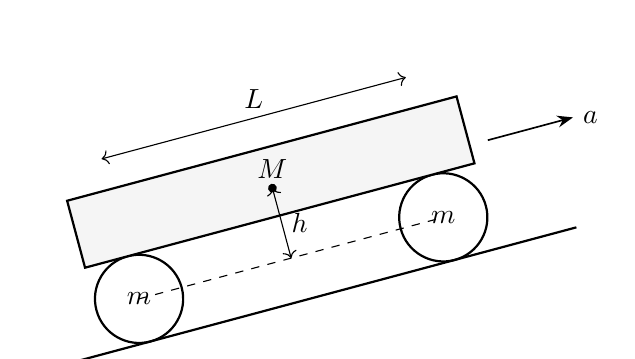
\begin{tikzpicture}[scale=.8,rotate=15]
\draw[thick] (-1,0)--(8,0);
\draw[thick] (1,.7) circle(.7);\draw[thick] (6,.7) circle(.7);
\draw[thick,fill=gray!8] (.3,1.4) rectangle(6.7,2.5);
\fill (3.5,1.85) circle(2pt) node[above] {$M$};
\draw[dashed] (1,.7)--(6,.7);
\draw[<->] (1,3)--(6,3) node[midway,above] {$L$};
\draw[<->] (3.5,.7)--(3.5,1.85) node[midway,right] {$h$};
\node at (1,.7) {$m$};\node at (6,.7) {$m$};
\draw[arr] (7,1.7)--(8.4,1.7) node[right] {$a$};
\end{tikzpicture}
}
\ifdim\wd\diagrambox>.88\linewidth
\sbox{\diagrambox}{\resizebox{.88\linewidth}{!}{\usebox{\diagrambox}}}\fi
\ifdim\ht\diagrambox>.20\textheight
\resizebox{!}{.20\textheight}{\usebox{\diagrambox}}
\else\usebox{\diagrambox}\fi
\par\smallskip{\small 图7a　车身高度h从轮轴平面量起\par}\endgroup\end{minipage}\end{center}

（1）汽车在倾角\(\theta\)坡面上无滑动地向上加速，加速度\(a\)，前、后轮法向力均大于零。求\(N_{\text{前}},N_{\text{后}}\)及不使前轮离地的最大安全加速度\(a_{\text{安全}}\)。

（2）车身发动机给后轮瞬时力矩\(\tau_{\text{轮}}\)，摩擦足以维持无滑动，求加速度。

（3）传动效率100\%，电机转速是车轮转速的\(r_i\)倍。A型车参数：\(M=1.8\times10^3\)
kg，\(h=0.1\) m，\(r=0.40\) m，\(L=2.9\)
m，电机最大转矩\(\tau=4.0\times10^2\)
N·m，\(r_i=10\)，轮质量可忽略，\(g=9.8\,\mathrm{m/s^2}\)。求水平和\(30^\circ\)上坡最大加速度、所需最小摩擦系数，数值保留两位有效数字。

\clearpage

\section{第 8
题　直流电机驱动的加速与能量效率（40分）}\label{ux7b2c-8-ux9898-ux76f4ux6d41ux7535ux673aux9a71ux52a8ux7684ux52a0ux901fux4e0eux80fdux91cfux6548ux738740ux5206}

简化电动车的前、后轮各视为半径\(r\)、质量\(m\)的均质圆柱，车身质量\(M\)，质心位于两轮轴中点正上方，轴距\(L\)。忽略空气阻力、轴承摩擦力矩，车轮惯量\(J_w=mr^2/2\)。

（1）简化永磁直流电机的线圈导线始终垂直切割匀强磁场\(B\)，有效切割导线总长\(l\)，转动轨迹半径\(r_{\text{线圈}}\)，线圈电阻\(R_{\text{线圈}}\)、自感可忽略。电池开路电压\(V\)、内阻\(R_{\text{内}}\)。无电机机械摩擦，求输出转矩\(\tau(\omega)\)、最大转矩\(\tau_{\max}\)、零功率空载最大转速\(\omega_{\max}\)及最大输出功率\(P_{\max}\)；用后三个量表示转矩曲线。

\begin{center}
\begin{minipage}{\linewidth}
\centering\begingroup\sbox{\diagrambox}{\small
\begin{tikzpicture}[scale=1]
\draw[thick] (0,0) rectangle(6,2);
\draw[fill=white] (.7,-.3) rectangle(1.9,.3);\node at (1.3,0) {$R_\Sigma$};
\draw[fill=white] (3,-.3) circle(.5);\node at (3,0) {$\mathcal E$};
\draw[fill=white] (4.5,-.3) rectangle(5.5,.3);\node at (5,0) {$V$};
\draw[arr] (1,2)--(2.5,2) node[midway,above] {$I$};
\node at (3,1.2) {$\mathcal E=K\omega,\quad\tau=KI$};
\node at (3,-1.1) {反电动势抵消部分电源电压};
\end{tikzpicture}
}
\ifdim\wd\diagrambox>.88\linewidth
\sbox{\diagrambox}{\resizebox{.88\linewidth}{!}{\usebox{\diagrambox}}}\fi
\ifdim\ht\diagrambox>.20\textheight
\resizebox{!}{.20\textheight}{\usebox{\diagrambox}}
\else\usebox{\diagrambox}\fi
\par\smallskip{\small 图8a　电源、总电阻与反电动势\par}\endgroup\end{minipage}\end{center}

（2）平地从\(t=0\)静止启动，车轮无滑动。已知\(a=(\tau_{\text{轮}}/r)/(M+3m)\)，传动效率100\%，电机转速为车轮的\(r_i\)倍，求\(v(t)\)。

（3）A型车\(M=1.8\times10^3\) kg，\(r=0.40\) m，\(L=2.9\)
m，\(\tau_{\max}=4.0\times10^2\)
N·m，\(r_i=10\)，轮质量忽略。电机\(P_{\max}=2.0\times10^2\)
kW。求从静止加速到\(v_f=100\)
km/h的时间、耗电池能量（kWh）及转化为机械能的效率。结果保留两位有效数字。

\end{document}
